In this section, we evaluate the performance of the proposed framework. Our
prototype of the framework has been implemented in the Go programming language
\cite{go}. The implementation comprises multiple independent libraries, and the
corresponding source code is available online \cite{sources}. The source code of
the experimental setup below along with all the configuration files and input
data is available at \cite{sources} as well. The experiments are conducted on a
laptop equipped with four processors Intel Core i7 2.5~\abbr{GH}z and
16~\abbr{GB} of \abbr{RAM}.

We shall consider $3 \times 2 \times 3 = 18$ uncertainty-quantification
problems. There are three platform sizes $\np$: 2, 4, and 8 processing elements;
there are two application sizes $\nt$: 10 and 20 tasks; and there are three
quantities of interest $\g$: the end-to-end delay, total energy, and maximum
temperature, which are given by \eref{end-to-end-delay}, \eref{total-energy},
and \eref{maximum-temperature}, respectively.

A platform with $\np$ processing elements and an application with $\nt$ tasks
are generated randomly by the \abbr{TGFF} tool \cite{dick1998}. The tool
generates $\np$ tables and a directed acyclic graph with $\nt$ nodes. Each table
corresponds to a processing element, and it describes certain properties of the
tasks when they are mapped to that particular processing element. Namely, each
table assigns two numbers to each task: a reference execution time, chosen
uniformly between 10 and 50~ms, and a power consumption, chosen uniformly
between 5 and 25~W. The graph captures data dependencies between the tasks. The
application is scheduled using a list scheduler \cite{adam1974}. The mapping of
the application is fixed and obtained by scheduling the tasks based on their
reference execution times and assigning them to the earliest available
processing elements (a shared ready list).

The construction of thermal \abbr{RC} circuits needed for temperature analysis
is delegated to the HotSpot tool \cite{skadron2004}. The floorplan of each
platform is a regular grid wherein each processing element occupies $2 \times
2~\text{mm}^2$ on the die. The output of the tool is essentially a pair of a
thermal capacitance matrix $\mC$ and a thermal conductance $\mG$ matrix used in
\eref{thermal-system}. The leakage power is not considered in these experiments,
which is solely for the sake of simplicity and is not required by our framework.

\begin{figure}[t]
  \centering
  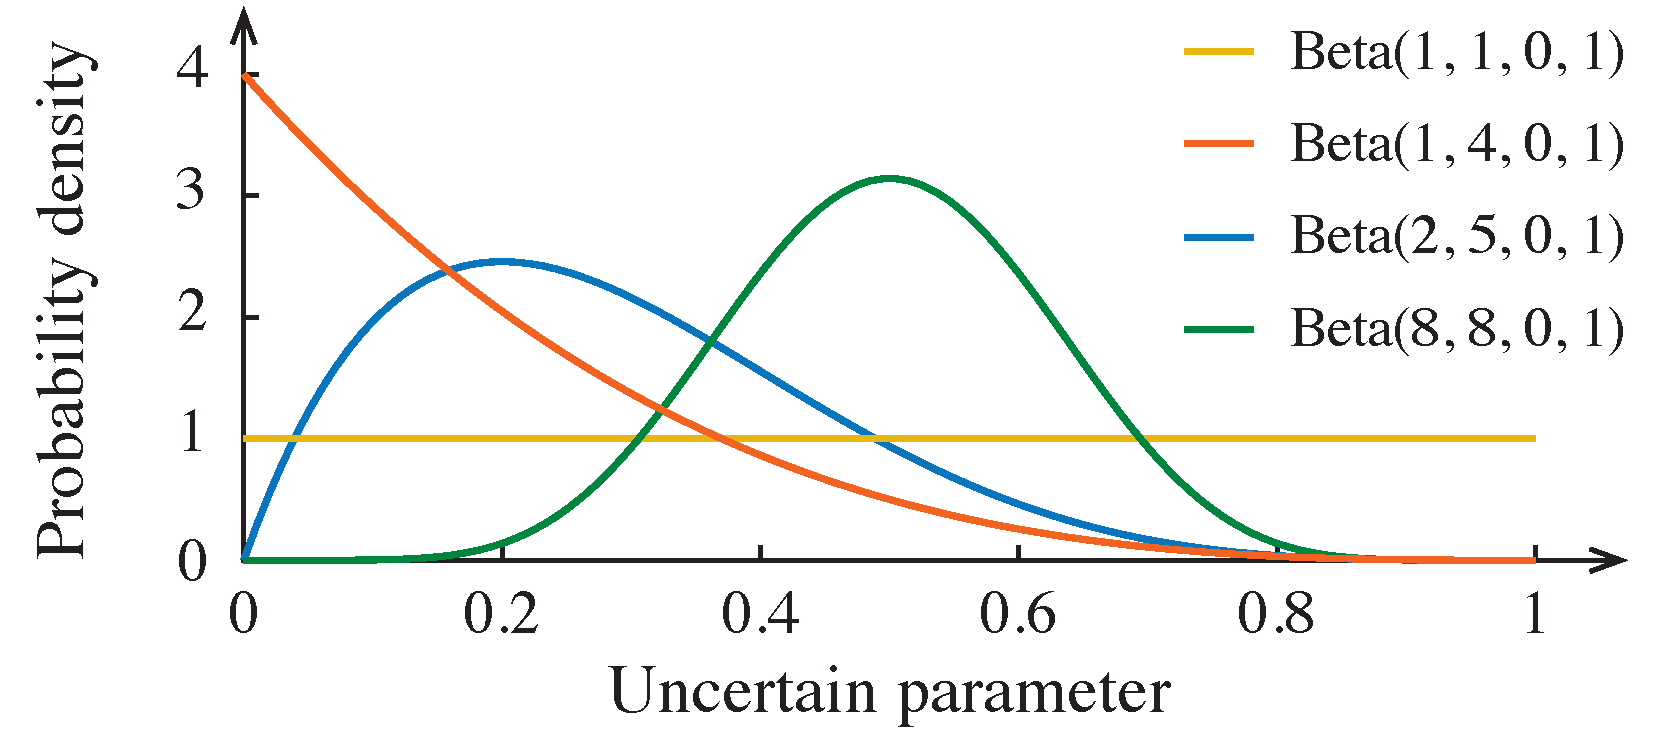
\includegraphics[width=1.0\columnwidth]{include/assets/figures/distribution.pdf}
  \caption{An illustration of the family of beta distributions.}
  \flab{distribution}
\end{figure}

The uncertain parameters $\vu$ are the execution times of the tasks; all other
parameters are deterministic. Targeting the practical scenario described in
\sref{uncertain-parameters}, the marginal distributions and correlation matrix
of $\vu$ are assumed to be available. Without loss of generality, the marginal
of $\u_i$ is a four-parametric beta distribution $\text{Beta}(\alpha_i, \beta_i,
a_i, b_i)$ where $\alpha_i$ and $\beta_i$ are the shape parameters, and $a_i$
and $b_i$ are the endpoints of the support. This family of distributions is very
reach; \fref{distribution} illustrates how the density function changes
dramatically depending on $\alpha_i$ and $\beta_i$. The left endpoint $a_i$ is
set to the reference execution time generated by the \abbr{TGFF} tool as
discussed earlier, and the right endpoint $b_i$ is set to be 20\% larger than
$a_i$. The parameters $\alpha_i$ and $\beta_i$ are set to two and five,
respectively, for all tasks, skewing their uncertain execution times towards the
reference execution times (the blue curve in \fref{distribution}). The execution
times of the tasks are correlated based on the structure of the graph produced
by the \abbr{TGFF} tool: the closer the $i$th and $j$th tasks are in the graph
as measured by the number of edges between the $i$th and $j$th nodes, the
stronger $\u_i$ and $\u_j$ are correlated.

Regarding the interpolation algorithm, we rely on the open Newton--Cotes rule as
motivated in \sref{collocation-nodes}. The \token{IsEnough} subroutine of
\aref{construct} terminates the algorithm when it reaches a certain
interpolation level. The decision taken in \token{IsAccurate} is based on the
formula given in \eref{error}.

In order to assess the performance of our framework, we shall compare the
results deliver by the framework with those delivered by a method based on
applying Monte Carlo (\abbr{MC}) sampling directly. The \abbr{MC} method
evaluates the quantity of interest $\g$ at a set of points drawn independently
from $\distribution_\vu$, the distribution of the uncertain parameter $\vu$. No
model order reduction is perform inside the \abbr{MC} method so that the
accuracy is not compromised by this reduction. The number of \abbr{MC}
simulations is set to $10^4$ for all experiments.

The main indicator of the efficiency of the proposed framework is the number of
evaluations of the quantity of interest needed to achieve a certain accuracy
level. Apropos accuracy, as noted \sref{introduction}, we are interested in
probability distributions and, therefore, shall report our accuracy of
estimating the distribution function of $\g$, $\distribution_\g$. (Other
quantities such as probabilistic moments are subordinate, and their accuracy can
be reasoned about using the accuracy of the distribution function as a proxy.)
The estimation of $\distribution_\g$ by sampling the constructed interpolant.

For comparing the proximity between two distribution, we shall use the
well-known Kolmogorov--Smirnov statistic \cite{rao2009}, which is the supremum
over the distance between two empirical distribution functions. The accuracy
metric is denoted by $\error$.

Lastly, we would like to remind that our setup is publicly available
\cite{sources}. The configuration aspects that have not been explicitly
mentioned here, such as the configuration files of the \abbr{TGFF} and HotSpot
tools, can be found online.

\begin{figure*}
  \vspace{-1.5em}
  \centering
  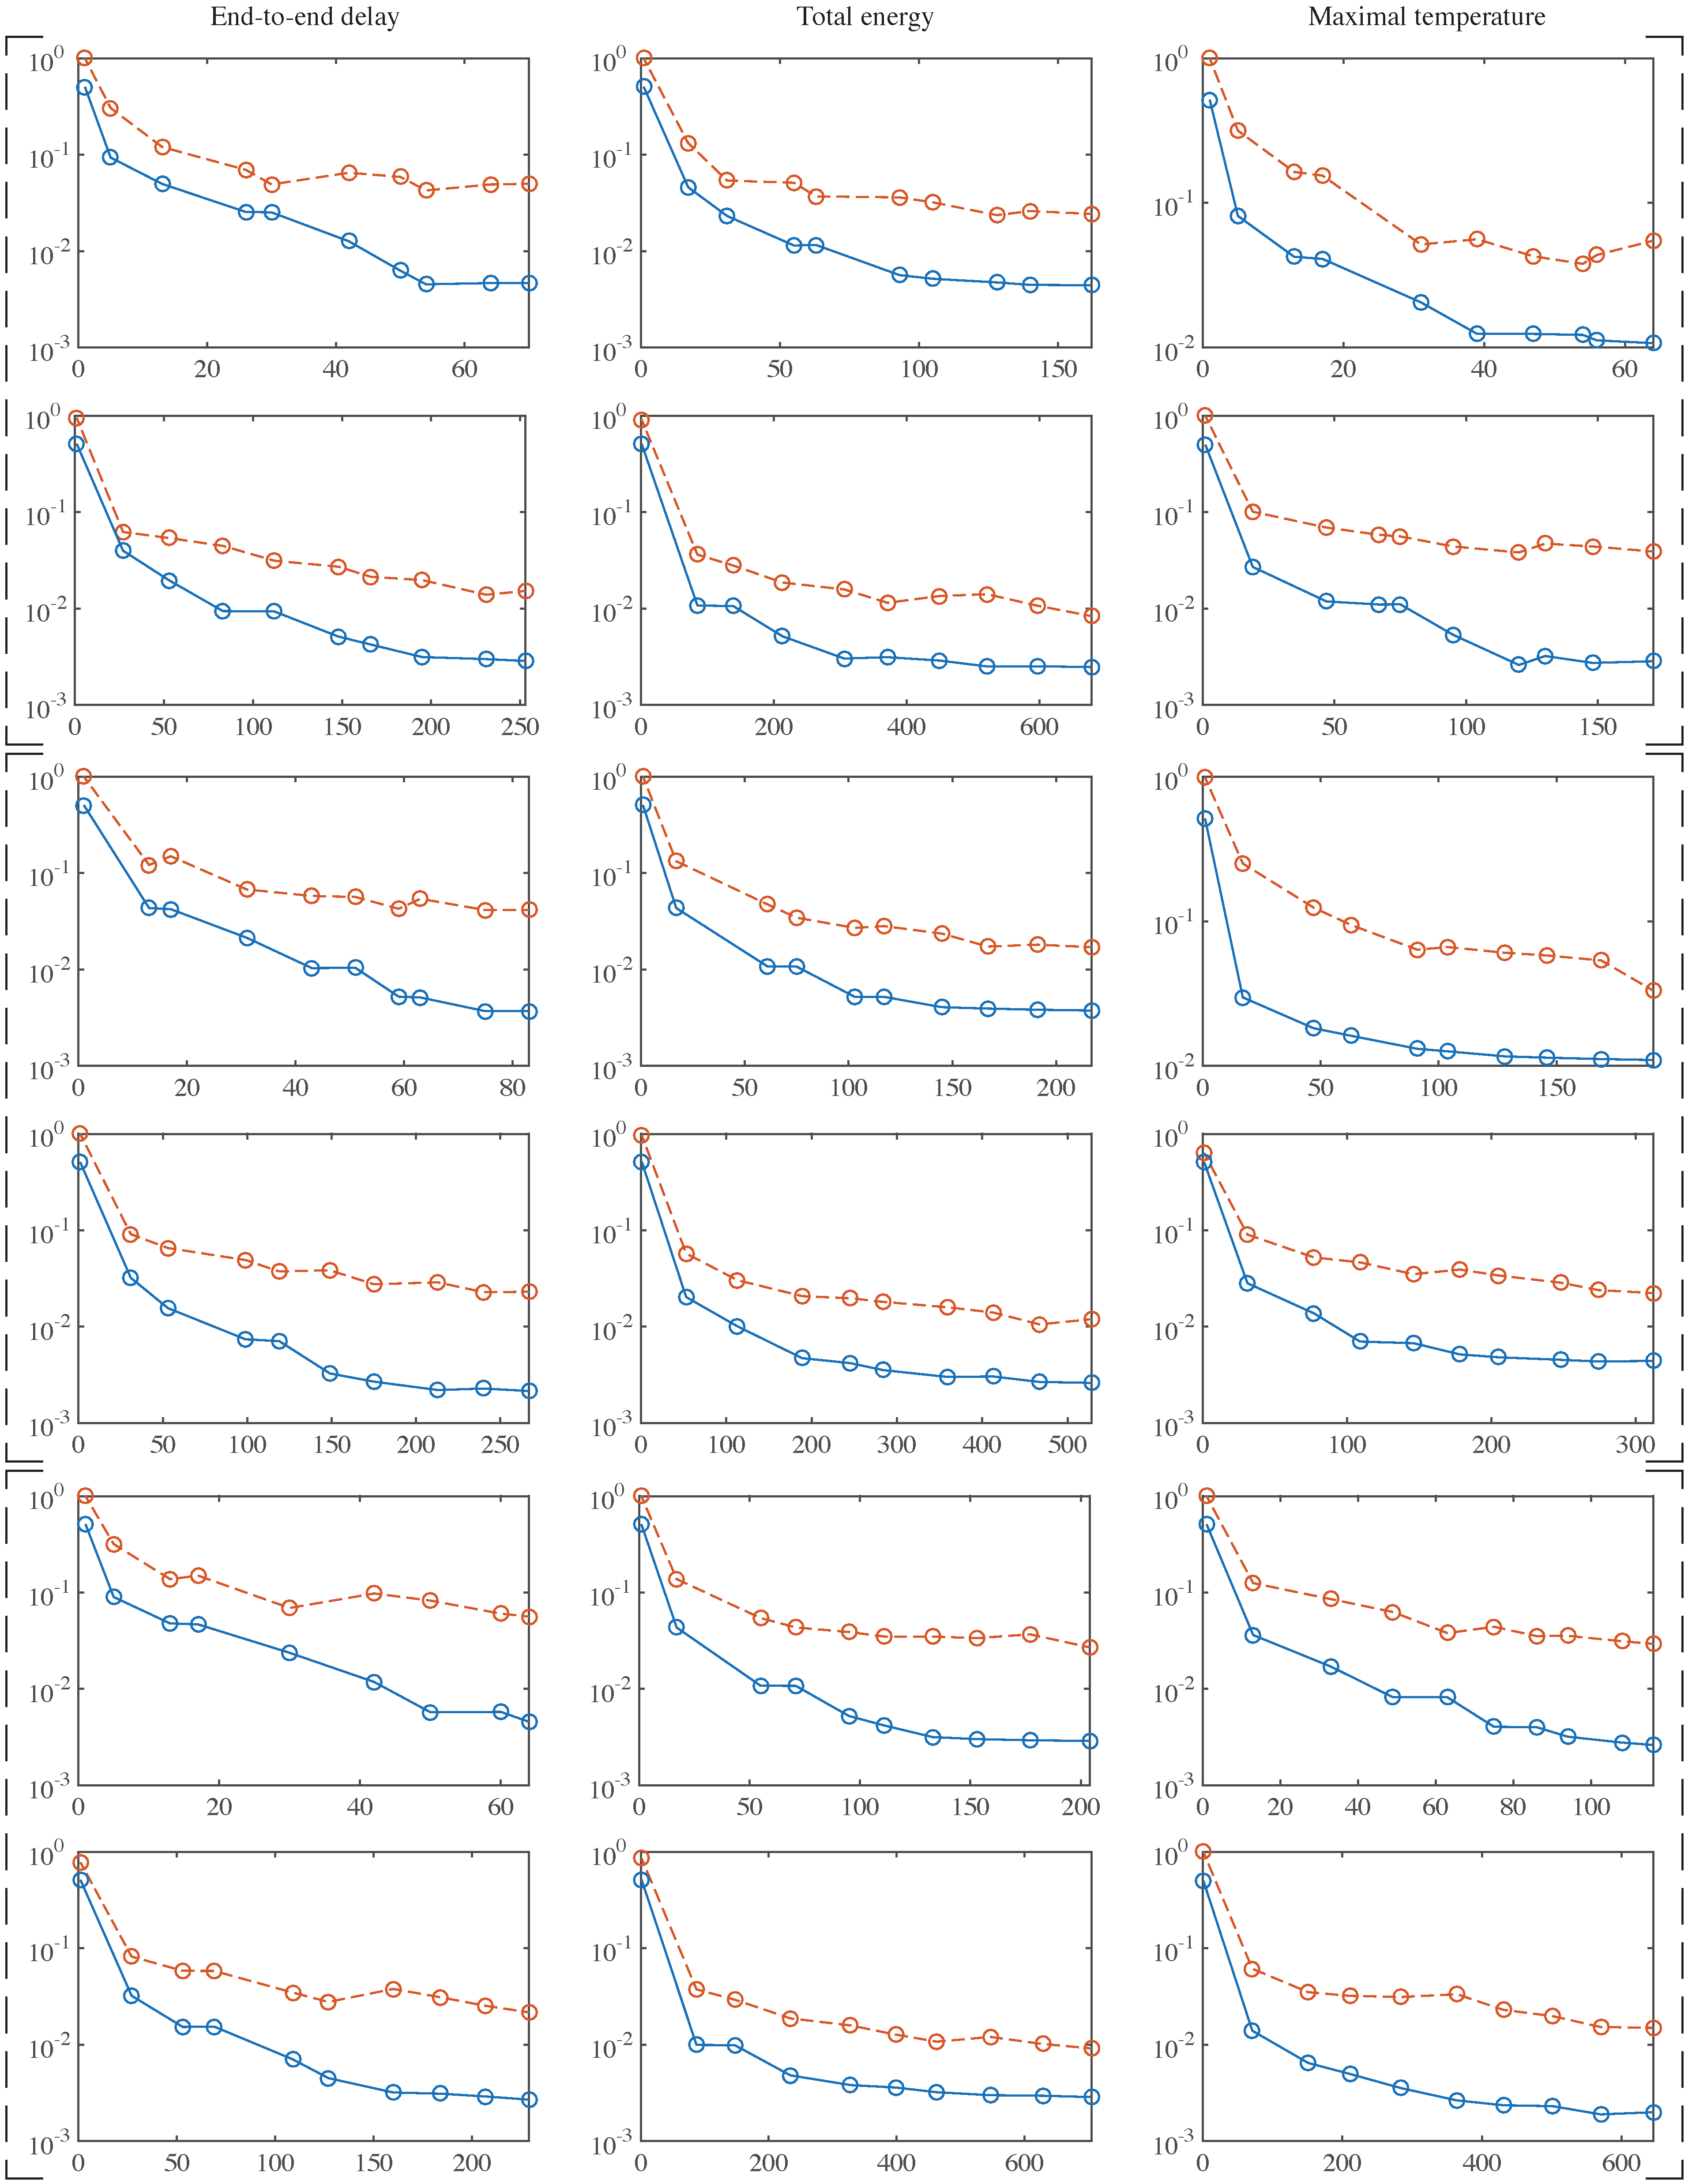
\includegraphics[width=1.0\textwidth]{include/assets/figures/results.pdf}
  \vspace{-1.5em}
  \caption{
    Experimental results. There are considered 3 quantities, 3 platform sizes,
    and 2 application sizes. The columns correspond to the three quantities: the
    end-to-end delay (left), total energy (middle), and maximum temperature
    (right). The three pairs of rows correspond to the three platform sizes: 2
    (top), 4 (middle), and 8 (bottom) processing elements. The rows alternate
    between the two application sizes: 10 (odd) and 20 (even) tasks. The
    horizontal axes show the number of points, and the vertical ones the error
    on a logarithmic scale. The solid lines correspond to our technique, and the
    dashed ones to direct sampling.
  }
  \flab{results}
\end{figure*}

\subsection{End-to-End Delay}
The quantity of interest $\g$ considered in this subsection is the end-to-end
delay given by \eref{end-to-end-delay}.

\subsection{Total Energy}
Let the quantity of interest $\g$ be the total energy given by
\eref{total-energy}.

\subsection{Maximum Temperature}
In this subsection, the quantity of interest $\g$ is the maximum temperature
given by \eref{maximum-temperature}.
